\begin{proof}
Soit $C$ une courbe. 
Soit $\epsilon>0$.
Soit \[A=\inf \enstq{B(i, \frac{\epsilon}{2})}{C\subset \bigcup_{icIcR2} B(i, \frac{\epsilon}{2})}\]
On note \[N_\epsilon =card(A)\]
Soit \[M_a (C)=\lim\limits_{\epsilon\rightarrow0}(N_\epsilon\epsilon^{a}), a\geq0, \textm{la mesure de Hausdorff}\]
On note: \[D_{H}(\mathcal{C})=\inf_{\mathbb{R}_{+}} \enstq{a}{Ma(\mathcal{C})=0}\]
Soit $\mathcal{Q}$ un quadrillage dont les cases, (notées $Q_{ij}, i,j e Z$) ont pour côté $\epsilon$.
Soit \[\mathcal{A'}= \enstq{Q_{ij}}{\mathcal{C}\subset \bigcup_{i,j e Z^{2}}Q_{ij}}\]
On note : \[N'_{\epsilon}=card(\mathcal{A'})\]
Soit \[\mathcal{M}_{a}'(\mathcal{C})=\lim\limits_{\epsilon\rightarrow0}(N'_\epsilon\epsilon^{a})\]
On note: \[D_{H}'(\mathcal{C})=\inf_{\mathbb{R}_{+}} \enstq{a}{Ma'(\mathcal{C})=0}\]
Objectif: Montrer que pour un $\mathcal{C}$ donné, \[D_{H}(\mathcal{C})=D_{H}'(\mathcal{C})\]
c'est à dire:\[\forall a \in IR+, \mathcal{M}_{a}(\mathcal{C})=0\Leftrightarrow \mathcal{M}_{a}'(\mathcal{C})\]
Prouvons maintenant que \[\mathcal{M}_{a}(\mathcal{C})=0 \Rightarrow \mathcal{M}_{a}'(\mathcal{C}) \]
c'est à dire \[\lim\limits_{\epsilon\rightarrow0}(N_\epsilon\epsilon^{a})=0 \Rightarrow \lim\limits_{\epsilon\rightarrow0}(N'_\epsilon\epsilon^{a})=0\]
Or \[\exists>0 | N'_{\epsilon} \leq cN_{\epsilon} \Rightarrow \lim\limits_{\epsilon\rightarrow0}(N_\epsilon\epsilon^{a})=0 \Rightarrow \lim\limits_{\epsilon\rightarrow0}(N'_\epsilon\epsilon^{a})=0\]
Or, \[\forall\epsilon > 0, N'_{\epsilon} \leq 4N_{\epsilon}\]
\begin{figure}[h]
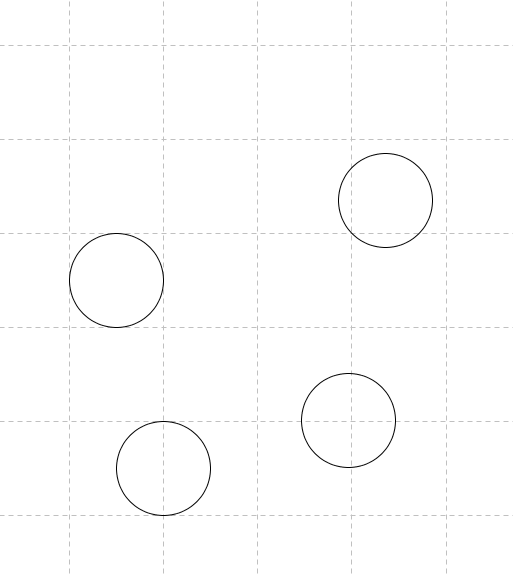
\includegraphics[width=10cm]{cases.png}
\caption{$\forall\epsilon > 0, N'_{\epsilon} \leq 4N_{\epsilon}$}
\label{fig:cases}
\end{figure}
Donc \[\lim\limits_{\epsilon\rightarrow0}(N'_\epsilon\epsilon^{a}) \leq \lim\limits_{\epsilon\rightarrow0}(4N_\epsilon\epsilon^{a})\]
c'est à dire \[\lim\limits_{\epsilon\rightarrow0}(N'_\epsilon\epsilon^{a}) \leq 4\lim\limits_{\epsilon\rightarrow0}(N_\epsilon\epsilon^{a})\]
c'est à dire \[\lim\limits_{\epsilon\rightarrow0}(N'_\epsilon\epsilon^{a}) \leq 0 \textm{(par hypothèse)}\]
Or 
\begin{equation*}
\begin{split}
N_{\epsilon}\geq 0 \textm{et}  \epsilon\geq0
& \Rightarrow 0 \leq \lim\limits_{\epsilon\rightarrow0}(N'_\epsilon\epsilon^{a}) \leq 0 \\
& \Rightarrow \lim\limits_{\epsilon\rightarrow0}(N'_\epsilon\epsilon^{a}) = 0 \textm{(selon le théorème de l'encadrement)}
\end{split}
\end{equation*}
Ainsi: \[\mathcal{M}_{a}(\mathcal{C})=0 \Rightarrow \mathcal{M}_{a}'(\mathcal{C})=0\]
Montrons que \[\mathcal{M}_{a}(\mathcal{C})=0 \Leftarrow \mathcal{M}_{a}'(\mathcal{C}) 
\lim\limits_{\epsilon\rightarrow0}(N_{\epsilon}\epsilon^{a})=0 \Leftarrow \lim\limits_{\epsilon\rightarrow0}(N'_{\epsilon}\epsilon^{a})=0\]
D'après la proposition, \[\exists c' | N_{c\epsilon} \leq N\epsilon' \Rightarrow (\lim\limits_{\epsilon\rightarrow0}(N'_\epsilon\epsilon^{a})=0 \Rightarrow \lim\limits_{\epsilon\rightarrow0}(N_\epsilon\epsilon^{a})=0)\]
Or \[N_{\sqrt{\epsilon}} \leq N'_{\epsilon}\]
Ainsi \[\lim\limits_{\epsilon\rightarrow0}(N_{\sqrt{\epsilon}^2}(\sqrt{\epsilon}^2)^{a}) \leq \sqrt[]{2}^{a}\lim\limits_{\epsilon\rightarrow0}N'_{\epsilon}\epsilon^{a}\]
Or \[N_{\sqrt{\epsilon}} \geq 0 \textm{et} (\sqrt[]{2}\epsilon)^{a} \geq0\]
On note \[\epsilon'=\sqrt[]{2}\epsilon\]
On voit que \[\epsilon'\rightarrow0 \Leftrightarrow \epsilon\Rightarrow0\]
Donc \[\lim\limits_{\epsilon\rightarrow0}(N_{\epsilon}\epsilon^{a})=\lim\limits_{\epsilon\rightarrow0}(N'_{\epsilon}\epsilon'^{a})=0\]
Ainsi \[\mathcal{M}_{a}(\mathcal{C})=0 \Leftrightarrow \mathcal{M}_{a}'(\mathcal{C})\]
Donc \[\inf_{\mathbb{R}_{+}}{\enstq{a}{M'_{a}(\mathcal{C})=0}}= \inf_{\mathbb{R}_{+}}{\enstq{a}{M_{a}(\mathcal{C})=0}}\]
Donc \[\mathcal{D}_{H}(\mathcal{C})=\mathcal{D}'_{H}(\mathcal{C})\]
\end{proof}